La verificación del sistema de Thary se llevó a cabo mediante pruebas automatizadas escritas con \textit{pytest}, ya explicadas en la Sección \ref{sec:verificacion_validacion}. Los resultados de estas pruebas se obtuvieron ejecutando el comando \texttt{pytest tests/ -v} en la terminal.

\begin{figure}[H]
    \centering
    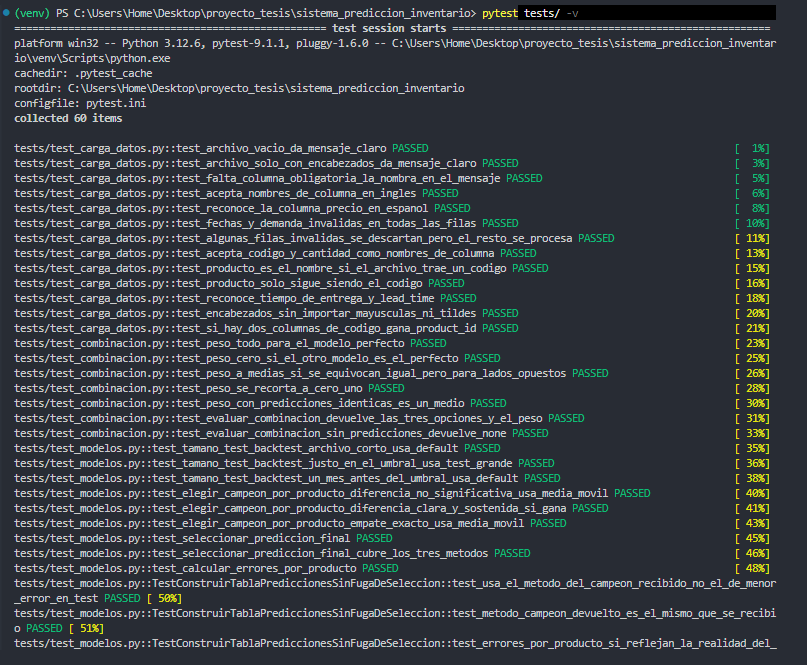
\includegraphics[width=\textwidth]{templatefigures/pytest_resultados_verbose}
    \caption{Ejecución detallada de la suite de pruebas mediante \texttt{pytest tests/ -v}, mostrando cada prueba individual.}
    \label{fig:pytest_verbose}
\end{figure}

\begin{table}[H]
    \centering
    \caption{Resultados de la suite de pruebas automatizadas por archivo.}
    \label{tab:resultados_pruebas}
    \renewcommand{\arraystretch}{1.3}
    \begin{tabularx}{\textwidth}{|l|X|c|}
    \hline
    \textbf{Archivo} & \textbf{Componente verificado} & \textbf{Resultado} \\
    \hline
    \texttt{test\_carga\_datos.py} & Carga y limpieza de datos, incluyendo el reconocimiento de columnas heterogeneas & 13/13 exitosas \\
    \hline
    \texttt{test\_combinacion.py} & Combinación de pronósticos & 7/7 exitosas \\
    \hline
    \texttt{test\_modelos.py} & Selección del modelo campeón y prueba Diebold-Mariano & 8/8 exitosas \\
    \hline
    \texttt{test\_reposicion.py} & Calculo de reposición (stock de seguridad, punto de reorden, EOQ, costo de ruptura) & 15/15 exitosas \\
    \hline
    \textbf{Total} & & \textbf{43/43 exitosas} \\
    \hline
    \end{tabularx}
\end{table}

\begin{figure}[H]
    \centering
    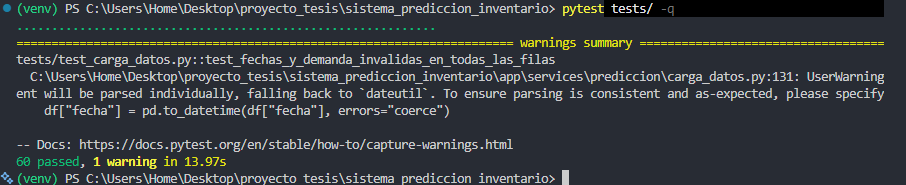
\includegraphics[width=0.8\textwidth]{templatefigures/pytest_resultados_resumen}
    \caption{Resumen final de la ejecución mediante \texttt{pytest tests/ -q}.}
    \label{fig:pytest_resumen}
\end{figure}

Como se puede ver en la Fig. \ref{fig:pytest_verbose}, la Tabla \ref{tab:resultados_pruebas} y la Fig. \ref{fig:pytest_resumen}, las 43 pruebas se ejecutaron correctamente en un tiempo de 5.56 segundos. Se registro una única advertencia (\textit{warning}) relacionada con el formato de fechas de pandas al procesar un archivo de prueba con fechas invalidas a proposito, sin que esto afecte el resultado de la prueba.


Se detecto un bug menor en el que la columna de "Precio" en español no era reconocida por el sistema a pesar de que la interfaz de carga la anunciaba como aceptada. Se arreglo el problema y dentro de \texttt{test\_carga\_datos.py} se incluyó la prueba \texttt{test\_reconoce\_la\_columna\_precio\_en\_espanol}, cuyo resultado exitoso confirma que la corrección aplicada sigue vigente.

El mecanismo de reconocimiento de columnas se reforzó con seis pruebas adicionales que verifican, entre otros casos: que el sistema ignore mayusculas y tildes en los encabezados, que resuelva correctamente la ambiguedad entre "Producto" como código o como nombre del producto (según si el archivo ya trae una columna de código clara), y que priorice la columna correcta cuando un archivo trae más de un candidato para el mismo destino (por ejemplo, un "Id" de transaccion junto a un "Product\_ID" real).
Además de las pruebas automáticas, se revisó de forma manual que la función principal de Thary se hiciera bien de principio a fin. Es decir, que el sistema dejara cargar un archivo, procesarlo, mostrar los resultados y confirmar un pedido sin errores. Las etapas de segmentación de productos, construcción de variables, y las rutas y autenticación de la aplicación web no tienen pruebas automáticas. Esto se reconoce como una limitación de la revisión.